\section{PCA}
PCA is a procedure which captures the directions of greatest data variability. That is, having a high dimensional dataset and performing an PCA would give us the eigenvectors and eigenvalues explaining the variance in the data. We can then choose to keep the eigenvectors that explain, say, 98\% of the variance in the data, and because the first few components / eigenvectors explain the vast majority of the variance, this will often lead to a big dimensionality reduction of the data.\\
In medical image analysis we can obtain such a high dimensionality dataset if we describe a shape by several data points / landmarks. If we were to describe a lung field, this could be done with 100 points in 2D giving us a 200 dimensional dataset for each lung field we describe. If we have several lung fields described in this manner, we can now normalize them using a Procrustes analysis and then perform PCA. In the data we are given, we have 124 lung fields described by 94 points. After performing PCA and retaining 98\% of the variance we find 20 components are enough. We can now visualize how adjusting the magnitude of the principal components affects our lungs. In \autoref{PCA} we see how the first three principal components affects our lung shape. These are the components which describes most of our variance in the data, and thus the components which gives the biggest change in shape.

\begin{figure}[h]
	\centering
	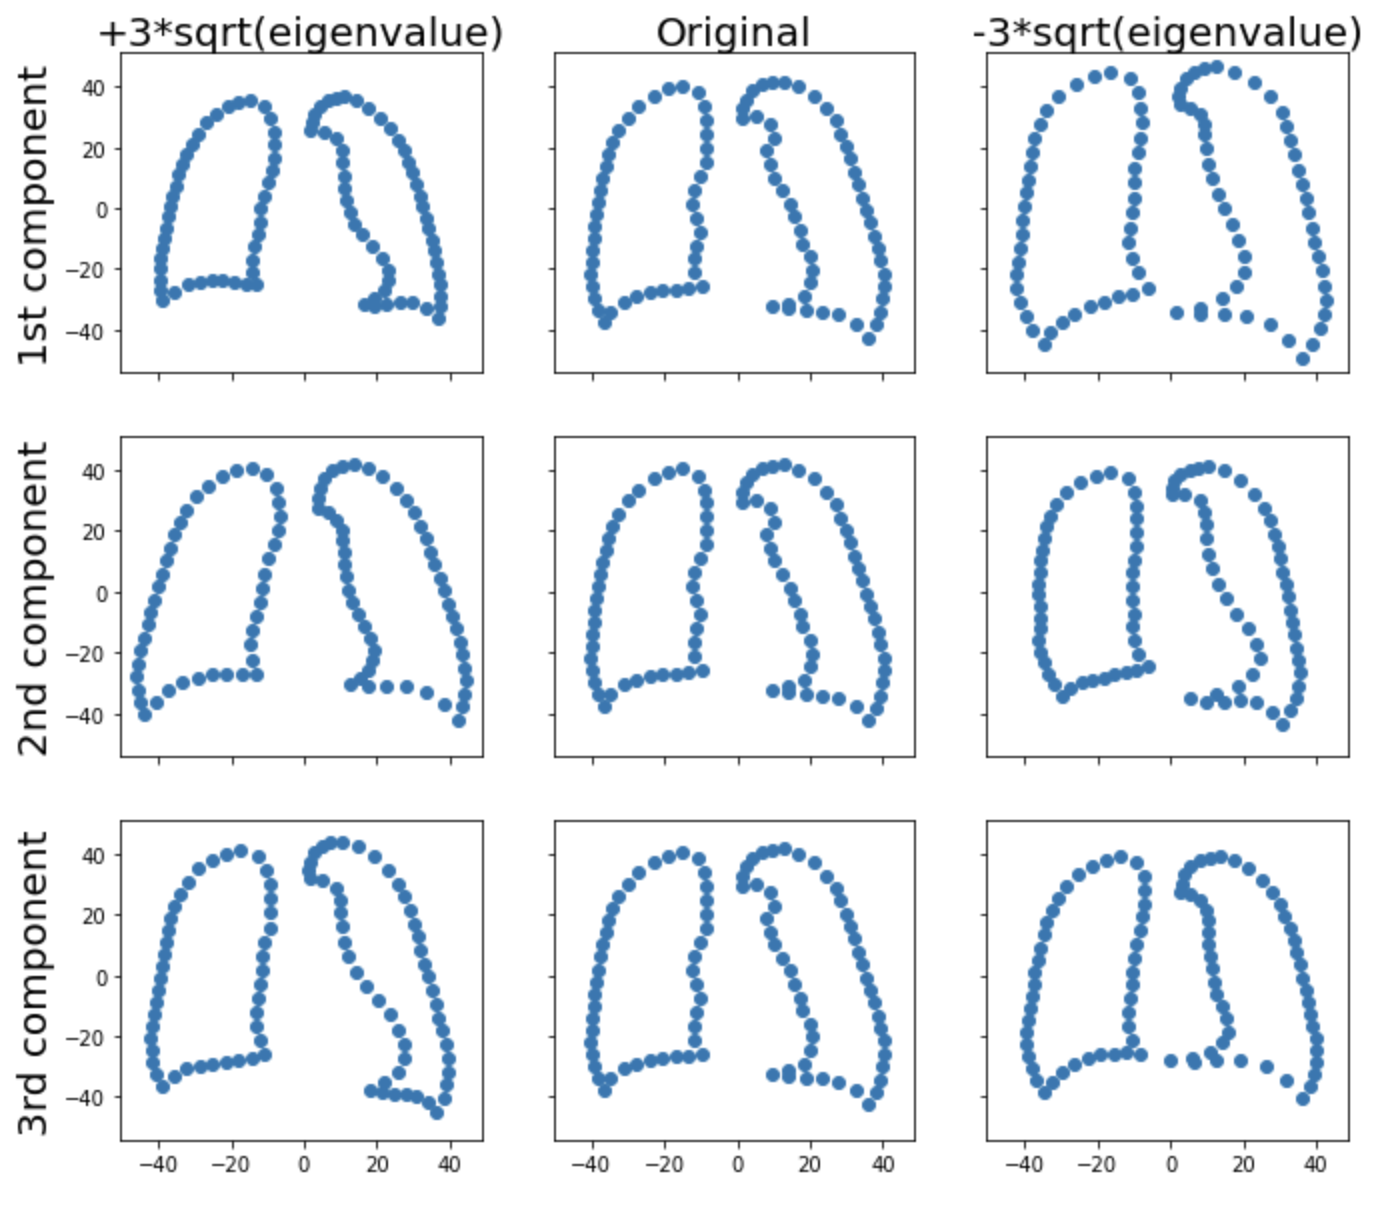
\includegraphics[width=0.73\linewidth]{Materials/PCA}
	\caption{How the first three principal components affects the shape of our lung.}
	\label{PCA}
\end{figure}
Using the 20 components describing 98\% of the variance in our lung fields we can now fit a mean lung shape, the lung found by taking the average shape of our lungs, to a never-before-seen lung and because we fit it using the components we avoid fitting to noise. We can then make an error measure of how well this active shape model / our mean lung fits our new lung, and use this to determine if we are seeing a healthy or sick lung / a normal or abnormal lung. Fitting our active shape model also gives a good boundary segmentation of the new lung. Even just using the mean lung shape would give a decent initial segmentation of a new lung field in most cases.